%--------------------------------------------------------------------------------------------------
\chapter{Einleitung} \label{cha:Einleitung}	

\lipsum[1]

%--------------------------------------------------------------------------------------------------
\section{Motivation}\label{sec:Motivation}

\lipsum[1]

%--------------------------------------------------------------------------------------------------
\section{Zielsetzung}\label{sec:Zielsetzung}
Das Ziel dieser Arbeit liegt in der Erschaffung eines Prototypen eines Menschmodells und einer Interaktionsschnittstelle um dem Menschmodell das interagieren mit der Umgebung zu ermöglichen. Dabei steht die Umgebung stellvertretend für den virtuellen Klon einer beliebigen Produktionsanlage. Weiterhin soll das entstandene Anwendungsbeispiel das Potenzial von Virtual Reality Technologien im Kontext von Industrie 4.0 darstellen.

%--------------------------------------------------------------------------------------------------
\section{Aufbau der Arbeit}\label{sec:AufbauDerArbeit}
Der Aufbau dieser Arbeit ist in Abbildung \ref{fig:AufbauDerArbeit} dargestellt.
\begin{figure}[h]
	\centering
	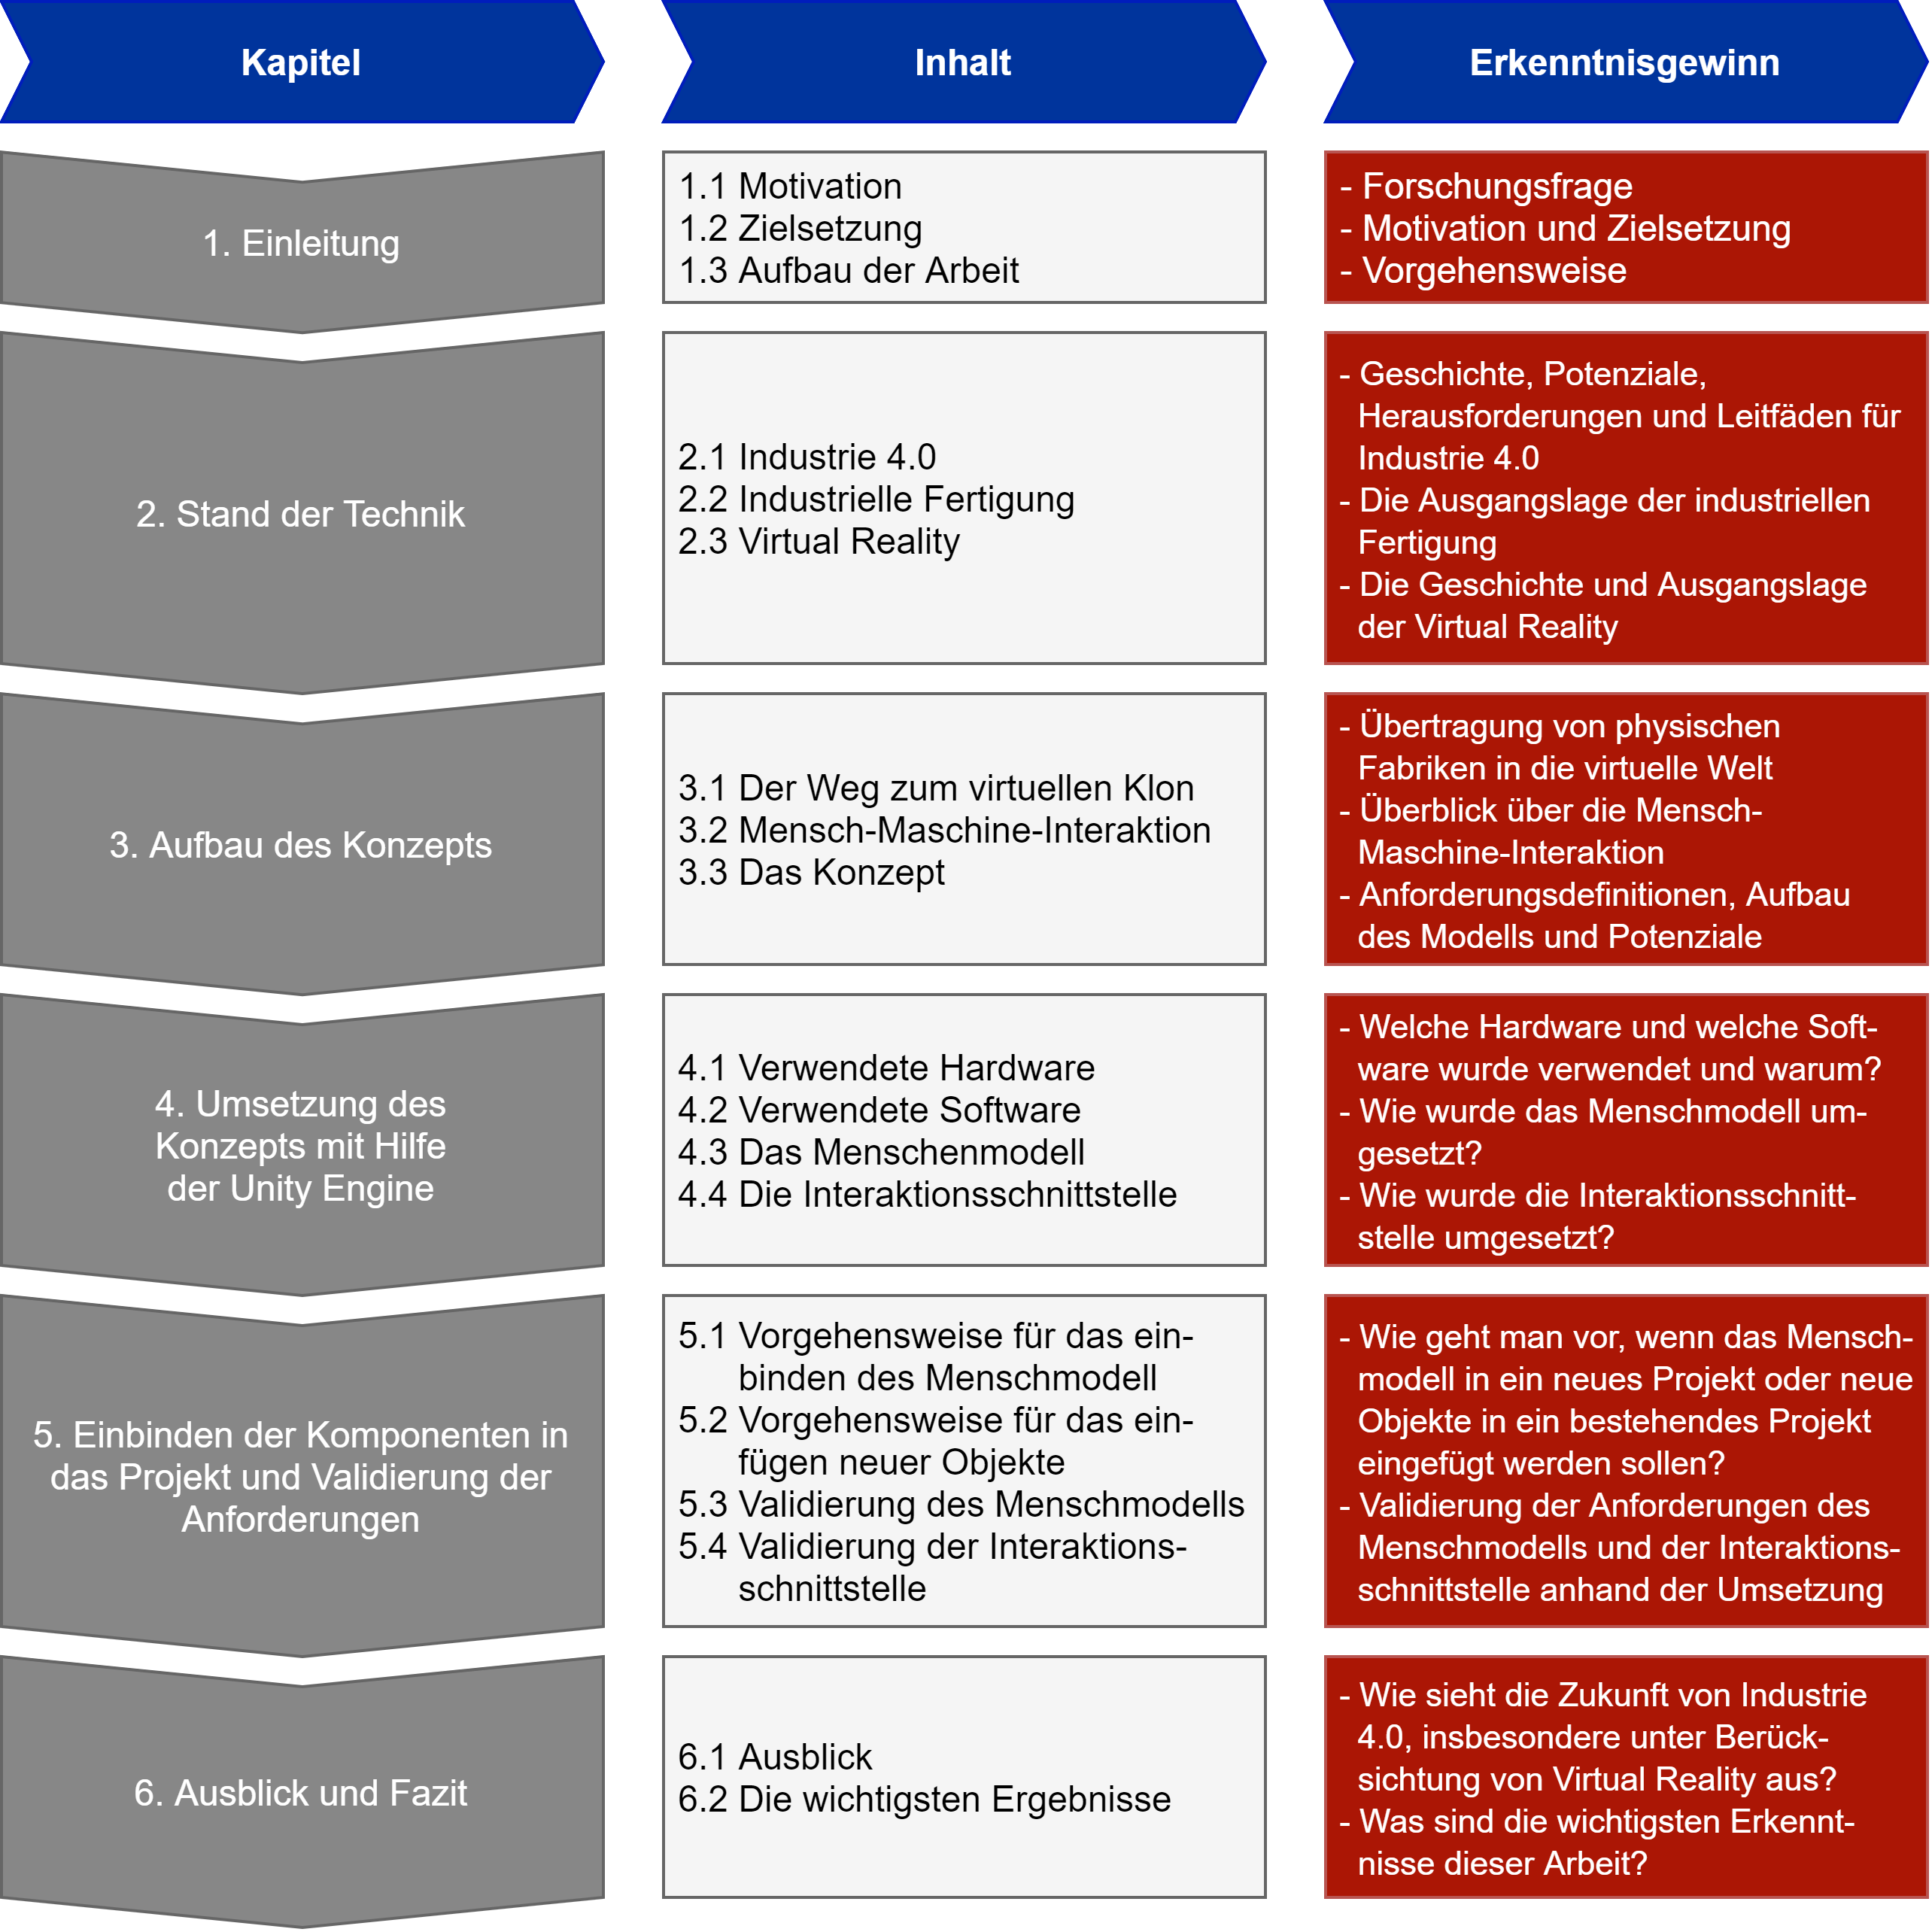
\includegraphics[width=1\linewidth]{Bilder/A55_AufbauNeu}
	\caption{Der Aufbau der Arbeit, eigene Abbildung}
	\label{fig:AufbauDerArbeit}
\end{figure}
\newline\newline
Zunächst wird, nach der Einleitung, in Kapitel \ref{cha:StandDerTechnik} der aktuelle Stand der Technik thematisiert. Aufgrund dessen gibt es in Unterkapitel \ref{sec:Industrie4.0} einen Einblick in die Geschichte der industriellen Revolutionen und der Wandlungen im Bereich der Informations- und Kommunikationstechnik (Kapitel \ref{sec:GeschichteIndustrie4}), bevor anschließend die Potenziale (Kapitel \ref{sec:PotentialeIndustrie4.0}) und Herausforderungen (Kapitel \ref{sec:HerausforderungenUmsetzung}) von Industrie 4.0 erläutert werden. Daraufhin werden noch zwei Leitfäden, die Unternehmen bei dem Wandel zu Industrie 4.0 unterstützten sollen (Kapitel \ref{sec:LeitfadenUmsetung}), erläutert. Anschließend gibt es in Unterkapitel \ref{sec:IndustrielleFertigung} noch eine Einführung in die Ausgangslage der industriellen Fertigung, insbesondere werden dabei der Produktlebenszyklus (Kapitel \ref{sec:Produktlebenszyklus}), die Automatisierungspyramide (Kapitel \ref{sec:Automatisierungspyramide}) und der Wandel der Automatisierungspyramide im Kontext von Industrie 4.0 (Kapitel \ref{sec:AutomatisierungspyramideUndIndustrie4.0}) erläutert. Zum Abschluss gibt es in Unterkapitel \ref{sec:VR} noch eine Einführung in das Thema virtuelle Realität, insbesondere in die Geschichte (Kapitel \ref{sec:VRGeschichte}) und die Potenziale (Kapitel \ref{sec:VRPotentialUndAusblick}) von Virtual Reality Technologien.
\newline
Im darauf folgenden Kapitel \ref{cha:AufbauDesKonzepts} wird das Konzept erläutert. Aufgrund dessen wird in Unterkapitel \ref{sec:PhysischZumKlon} zunächst der Prozess von der physischen Produktionsanlage bis hin zu ihrem virtuellen Klon erläutert und die Arbeit in diesem Prozess eingeordnet. Daraufhin gibt es in Unterkapitel \ref{sec:MMInteraktion} einen Überblick über die Mensch-Maschine-Interaktion im Kontext dieser Arbeit, bevor die Arbeit auch in diesem Kapitel entsprechend eingeordnet wird. Anschließend wird in Unterkapitel \ref{sec:ModellAufbau} das eigentliche Konzepts des Menschmodells aufgebaut, indem zunächst die Anforderungen an das Menschmodell und die Interaktionsschnittstelle erläutert werden (Kapitel \ref{sec:AnforderungenKonzept}). Des Weiteren gibt es eine Einführung in das Functional-Mockup Interface (Kapitel \ref{sec:DasFMU}), bevor erläutert wird, wie die Umsetzung des Menschmodells mit Hilfe des FMI Standards auszusehen hätte (Kapitel \ref{sec:ModelAufbau}) und worin die Potenziale liegen würden (Kapitel \ref{sec:PotenzialeFMU}).
\newline
Aufbauend auf dem im vorherigen Kapitel gewonnen Verständnis und insbesondere unter Berücksichtigungen der gestellten Anforderung an das Menschmodell und die Interaktionsschnittstelle, wird in Unterkapitel \ref{cha:Umsetzung} die Umsetzung des Konzepts mit Hilfe der Unity Engine erläutert. Aufgrund dessen gibt es in Kapitel \ref{sec:Hardware} zunächst eine Einführung in die Verwendete Hardware. Dazu gehören die Brille und ihr Zubehör (Kapitel \ref{sec:GrundHardware}), die Tracker (Kapitel \ref{sec:TrackerVive}) und auch die Befestigungen für die Tracker (Kapitel \ref{sec:TrackerBefestigung}). Daraufhin wird in Unterkapitel \ref{sec:Software} die verwendete Software, also die VIVE Wireless Anwendung (Kapitel \ref{sec:VIVEWireless}), die SteamVR Anwendung (Kapitel \ref{sec:SteamVR}) und die Entwicklungsumgebung Unity Engine mit den genutzten Plugins (Kapitel \ref{sec:UnitEngine}), erläutert. Anschließend wird in Unterkapitel \ref{sec:DasMenschmodell} die Umsetzung des Menschmodells erklärt, vom Grundgerüst des Menschmodells (Kapitel \ref{sec:MMModell}), über die ergänzenden Komponenten (Kapitel \ref{sec:MMKomponenten}) und erstellten Skripte (Kapitel \ref{sec:MMCode}), bis hin zu einer kurzen Zusammenfassung des entstandenen Modells (Kapitel \ref{sec:MMFunktionen}). Schließlich wird in Unterkapitel \ref{sec:DieInteraktionsschnittstelle} die Umsetzung der Interaktionsschnittstelle erläutert. Daher werden zunächst das Grundgerüst (Kapitel \ref{sec:GrundgerüstInteraktion}), daraufhin die ergänzenden Komponenten (Kapitel \ref{sec:WeitereTeileInteraktion}) und anschließend eine kurze Zusammenfassung der entstandenen Interaktionsschnittstelle (Kapitel \ref{sec:ZusammenfassungInteraktion}) vorgestellt.
\newline
In Kapitel \ref{cha:ValidierungDesKonzepts} gibt es zunächst im Unterkapitel \ref{sec:MenschmodellEinbinden} eine Einführung in die Vorgehensweise beim Einbinden des Menschmodells und der Interaktionsschnittstelle in ein neues Projekt (Kapitel \ref{sec:MenschmodellEinbinden1} - \ref{sec:MenschmodellEinbinden3}), bevor anschließend in Unterkapitel \ref{sec:ObjekteEinbinden} die Vorgehensweise beim Einfügen neuer Objekte in der Umgebung erläutert wird (Kapitel \ref{sec:ObjekteEinbinden1} - \ref{sec:ObjekteEinbinden3}). Schließlich werden in Unterkapitel \ref{sec:ValidMensch} (\ref{sec:ValidMensch1} - \ref{sec:ValidMensch4}) und \ref{sec:ValidInteraktion} (\ref{sec:ValidInteraktion1} - \ref{sec:ValidInteraktion5}) die gestellten Anforderungen an das Menschmodell und die Interaktionsschnittstelle, unter Berücksichtigung der erläuterten Umsetzung des Konzepts mit Hilfe der Unity Engine, validiert.
\newline
Abschließend gibt es in Kapitel \ref{cha:AusblickUndFazit} in Unterkapitel \ref{sec:Ausblick} einen Ausblick, der sich damit befasst, wie die Zukunft von Industrie 4.0, insbesondere im Hinblick auf Virtual Reality, aussehen könnte, bevor in Unterkapitel \ref{sec:ZusammenfassungErgebnisse} die wichtigsten Erkenntnisse der Arbeit zusammengefasst werden.

%--------------------------------------------------------------------------------------------------